% Generated by scripts/financial/build_pms_v2_release.py.
% Validation-only evidence. Do not describe these results as locked-test performance.
% Requires the graphicx and booktabs packages.
\subsection{Validation-only PMS-Mamba optimization}
\label{sec:pms-v2-validation}

We evaluated eight prespecified PMS-Mamba configurations in a resolution-IV
fractional-factorial screen across eight forecasting tasks, three training seeds,
and six horizons. The two leading configurations were then evaluated with five
seeds and compared with the current PMS-Mamba configuration (F04) on the same
validation splits. F01 reduced mean balanced RMSSE by 1.79\% relative to F04
(descriptive 95\% paired bootstrap interval, 1.51\% to 2.02\%), whereas F03 reduced
it by 1.68\% (1.20\% to 2.13\%). These improvements did not meet the prespecified
2\% practical-effect threshold; therefore, F04 was retained and no new locked-test
evaluation was opened.

\begin{table}[t]
  \centering
  \caption{Five-seed validation confirmation of the two screened finalists. RMSSE
  is lower-is-better. Intervals are descriptive 95\% percentile intervals from
  10,000 paired bootstrap resamples of 40 task--seed validation summaries. The
  frozen success rule required at least 2\% overall improvement and no term-level
  degradation greater than 5\%.}
  \label{tab:pms-v2-validation}
  \begin{tabular}{lrrrr}
    \toprule
    Configuration & Mean RMSSE & Improvement & 95\% interval & Better runs \\
    \midrule
    F01 & 9.849 & 1.79\% & [1.51\%, 2.02\%] & 38/40 \\
    F03 & 9.859 & 1.68\% & [1.20\%, 2.13\%] & 28/40 \\
    F04 (reference) & 10.028 & 0.00\% & -- & -- \\
    \bottomrule
  \end{tabular}
\end{table}

The exploratory screen identified residual anchoring as the strongest favorable
factor. Its high-minus-low effect was $-1.77\%$ of the grand mean balanced RMSSE
(descriptive 95\% paired bootstrap interval, $-2.76\%$ to $-0.89\%$). Scale-normalized MSE was
unfavorable (6.11\%; 1.99\% to 10.96\%), while gated fusion and late-step weighting
had smaller average effects. Because the fractional design aliases main effects with
three-factor interactions, these estimates are diagnostic rather than confirmatory.

\begin{figure}[t]
  \centering
  % Add reproducibility/nonstationary_analysis_v2/analysis/ to \graphicspath.
  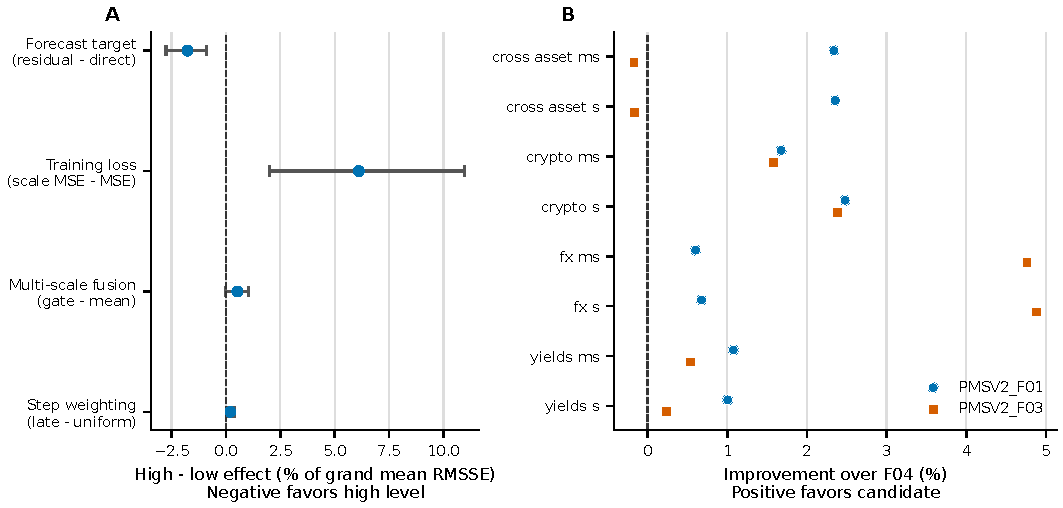
\includegraphics[width=\linewidth]{pms_v2_validation_effects.pdf}
  \caption{Validation-only PMS-Mamba V2 analysis. (A) High-minus-low factor effects
  on balanced RMSSE in 24 paired task--seed screening blocks; negative values favor
  the high factor level. Error bars are descriptive 95\% percentile intervals from
  10,000 paired bootstrap resamples. (B) Five-seed task-level improvement of F01 and
  F03 over F04; positive values favor the candidate. Color and marker shape jointly
  encode configuration. No protected test targets were used.}
  \label{fig:pms-v2-validation}
\end{figure}

Taken together, the validation study supports retaining residual anchoring as a
future design direction, but it does not support replacing the current PMS-Mamba
configuration under the frozen decision rule. A subsequent protocol should examine
long-horizon capacity or regime conditioning without reusing the protected test period
for model selection.
